\documentclass[runningheads,a4paper]{llncs}

\usepackage{amssymb}
\setcounter{tocdepth}{3}
\usepackage{graphicx}
\usepackage{subfigure}

\usepackage{url}
\newcommand{\keywords}[1]{\par\addvspace\baselineskip
\noindent\keywordname\enspace\ignorespaces#1}

\begin{document}

\mainmatter  % start of an individual contribution

% first the title is needed
\title{World building: analysing the parameters that for massive generation of coherent backstories in fiction environments}

% a short form should be given in case it is too long for the running head
\titlerunning{World building}

% the name(s) of the author(s) follow(s) next
%
%
\author{Non A. Me%
\thanks{NoInstitute}}
%
\authorrunning{Me, N}
% (feature abused for this document to repeat the title also on left hand pages)

% the affiliations are given next; don't give your e-mail address
% unless you accept that it will be published
\institute{No Institute}

%
% NB: a more complex sample for affiliations and the mapping to the
% corresponding authors can be found in the file "llncs.dem"
% (search for the string "\mainmatter" where a contribution starts).
% "llncs.dem" accompanies the document class "llncs.cls".
%

\maketitle


\begin{abstract}
Generating fictional worlds according to some specific requisites
presents the problem that it is impossible to know in advance the optimum for the
particular fitness function designed at the same time it creates a
vast search space for the evolutionary algorithm parameters that it
needs. In this paper our objective is to find a methodology for finding the
best parameters of the evolutionary algorithm in the design of
fictional worlds. This evolutionary design includes running, to
completion, a world represented as a chromosome and assigning a fitness to it, so it is a problem
with a very complex fitness landscape. That is why, in order to
optimize resources given to evolution and also have some guarantee
that the final result will be close to optimal, we systematically
study the values of different parameters to try and find a set of
rules that will, once you have the fitness function, help you set a
reduced range of values o even a single value that will, with a
reduced computation budget, help you find an optimal world.

\keywords{Games, Plot, evolutionary algorithms, content generation, literature}
\end{abstract}

\section{Introduction}

In the very competitive cultural industry, writers rack their minds in
order to generate interesting fictional worlds, mainly for the
creation of richer environments in modern videogames. In order to make
generation of these fictional worlds and the stories within them truly efficient and massive,
several methods have been proposed \cite{garcia14my,nairat:evolution}. One of them, called MADE
\cite{garcia14my} finds ``interesting'' character stories by running
an evolutionary algorithm that optimizes a fitness function designed
from the archetypes that best describe the world the client wants.

MADE works as follows: every individual in an evolutionary algorithm
is described by a chromosome that represents one (or several kinds of)
finite state automaton that are set to live in a simulated
environment. The evolutionary algorithm was run with standard
parameters and {\em sensible} default values were given to several
non-evolutionary parameters such as the number of profiles needed to
obtain the desired result and or the size of the simulated
world. There was no attempt to optimize these parameters, since the
main intention seemed to be to have a prototype that allowed the
authors to have an acid test of their proposed approach.

That paper hinted at the fact that parameters such as the number of
{\em profiles} (different kind of finite state automaton present in
the world) had a big influence on the outcome, to the point of making
it possible or not. However, other parameters such as the number of
simulated days the world is running might also have some influence.

In this paper we will use that open source simulator and look at it
from the evolutionary point of view so that we can check what kind of
influence they have in the outcome. We will do a experimental setup
that will test different parameters, and eventually find a series of
rules that will help the users of that framework to set the best
values for their simulation. 

The rest of the paper is organized as follows. Coming up next, we
present the state of the art in parameter setting of simulated
worlds. Next we will present the experimental setup we follow in this
article, whose results will be shown in Section \ref{sec:res}. Finally, we will
present the conclusions reached in this paper.

\section{State of the Art}

The work of Nairat et al. \cite{nairat:evolution} ...

\section{Methodology and experimental setup} %Issue #12
\label{sec:met}

In this section we will show how to systematize the different steps of the proposed method to generate a fictional world. Initially, the fitness should be decided considering the desired behaviour of the agents that populate the world (for example, a given quantity of some archetype). To facilitate the generation of different personalities different number of ``profile'' could be required. This concept, presented in \cite{}, describes the different sets of behaviour parameters of the agents in the world (the number of different FSMs). Therefore, a world with 3 profiles is composed by 3 different types of agents. However, and as will be probed in this paper, the number of profiles could be different of the number of desired archetypes.

Then, the characteristics of this world are also decided taking into account the expected... For example, adding enough days to allow the archetypes generation. Finally, the interesting plot points are extracted from the log using... 



In this work, we propose three scenarios:
\begin{itemize}
\item Scenario A: The Villains. This scenario only requires one type of archetype: The ``villain''. This 
\item Scenario B: The Hero. As in the classic stories, when a villain appears, a hero must rise. The ``hero'' archetype depend on the existence of a ``villain'' archetype. This scenario tries to generate worlds formed by archetypes that depend of anothers.
\item Scenario C: The Shakespearian story. As many of the great stories of The Bard, this world requires the existence of different and interdependant archetypes: The ``hero'' and ``villain'' are completed with the ``obstacle'' (QUE HACE QUE), the  ``mentor'' (QUE HACE QUE) and the ``avenger'' (this archetype does not depend on the others).
\end{itemize}

\subsection{Designing a fitness function}

The first step requires to develop a fitness function that takes into
account the quantity of the desired archetypes. This fitness function
should facilitate the existence of diversity in the desired
archetypes: that is, it is better that the world has 25\% of
``villains'' and 25\% of ``heroes'' than 50\% of ``villains'' and no
``heroes''. Thus, we propose the following fitness function: 

\begin{equation}
\sum _{i=1}^{P} {\log \left( 1+10p_{i}\right) } \over {\log 1}
\end{equation}

where $P$ is the number of desired profiles, and $p_{i}$ is the
percentage (from 0 to 1) of a specific profile in the world. % Why
                                % logs and all the rest? - JJ

In this paper, three fitness functions will be studied, related with the previously explained scenarios:
\begin{itemize}
\item Function 1: for the scenario A . This function requires the maximization of the ``villain'' archetype, trying to maximise the number of villains in the world. 
\item Function 2: for the scenario B. In this, case, the ``hero'' archetype... and villain ()
\item Function 3: for the scenario C... This function requires 5 different archetypes. These archetypes have some type of interdependence. hero villano obstaculo mentor y vengativo (este no deènde de nadie)
\end{itemize}

\subsection{Individual representation}

The number of profiles has a direct relation with the desired fitness functions. It is expected that functions with only one kind of archetype (such as F1 and F2) only would require one profile. Furthermore, the number of profiles affect the generated fitness as the chromo
% Chromo what?


\subsection{System optimization}


Once the fitness function has been decided, several parameters related with the world and the GA will be studied

The parameters of the world affect  % JUSTIFICAR ...


Number of days: 128, 256


Finally, the parameters of the GA also affect the execution of... the
population size ... 64, 128, 256 % JUSTIFICAR

As the usage of different number of profiles generate different
individual sizes, and therefore, different convergence times the stop
criterion has been established in... % TERMINA

Table \ref{tab:parameters} summarizes all the configuration parameters that will be compared, and the rest of the (fixed) parameters of the algorithm. The fixed values of the parameters of the GA have been usually described by other authors as...

\begin{table*}
\begin{center}
\begin{tabular}{|c|c|}
\hline
{\em Parameter} & {\em Values} \\\hline \hline
\multicolumn{2}{c}{Parameters under study} \\ \hline \hline
Number of profiles & 1, 2, 4 and 8 \\\hline
Number of virtual days &  128 and 256 \\ \hline
World dimension &  5x5, 10x10 and 20x20 \\ \hline
GA population size & 64, 128 and 256 \\ \hline
\multicolumn{2}{c}{Fixed parameters} \\ \hline \hline
Mutation probability & 1/12 per gene \\ \hline
Parent pool size & Same as pool size \\ \hline
Selection method & Binary tournament \\ \hline 
Elite & 10\%  \\ \hline
% Cuando algo no compile lo arregláis, no lo borréis!!!! - JJ
Replacement method & Generational\\ \hline
Stop condition & \\ \hline %Stop condition? - JJ
Runs per configuration & 30 \\ \hline
\end{tabular}
\caption{Parameters used in the experiments.}
\label{tab:parameters}
\end{center}
\end{table*}

%\subsection{Converting logs to stories}

% 12 pages is the limit. 
\section{Results}
\label{sec:res}


In this paper, 9720 runs were carried out for each problem (30 times * 4 levels for \emph{P} * 2 levels for \emph{D} * 3 levels for \emph{W} * 3 levels for \emph{S} * 3 levels for \emph{F} that represent the possible combinations) to obtain the fitness for each combination.


As the Kolmogorov-Smirnov test determines that the data we are using not follow a normal distribution a Kruskal–Wallis test have been performed. This test is a non-parametric test, which means that it does not assume that the data come from a normal distribution. 


The application of Kruskal-Wallis consisted in running the EA optimization method using those parameter combinations to obtain the best fitness. 
The response variable used to perform the statistical analysis is the fitness at the end of the run. The changes in the response variable are produced when a new combination of parameters is considered. Then, the {R} \footnote{{\tt http://www.r-project.org}} tool was used to obtain the Kruskal-Wallis tables as well as the tables of means and figures for each problem. 

Obtained Kruskal-Wallis tables show for each factor, the  degrees of freedom (FD), the experimental value of the statistical F (F value) and its associated p-value.
As previously stated, if the output is smaller than 0.05, then the factor effect is statistically significant at a $95\%$ confidence level (what indicates that different initial values of this parameter lead to significant differences on the fitness). 

As a significant F-value only tells  that the effects are not all equal (i.e., reject the null hypothesis), post-hoc tests might be used to determine which effects or outputs are significantly different from which other.

Results show that all the parameters considered have a significant impact in the generation of the agents.

\begin{figure}
        \centering
        \subfigure[Profiles]{
                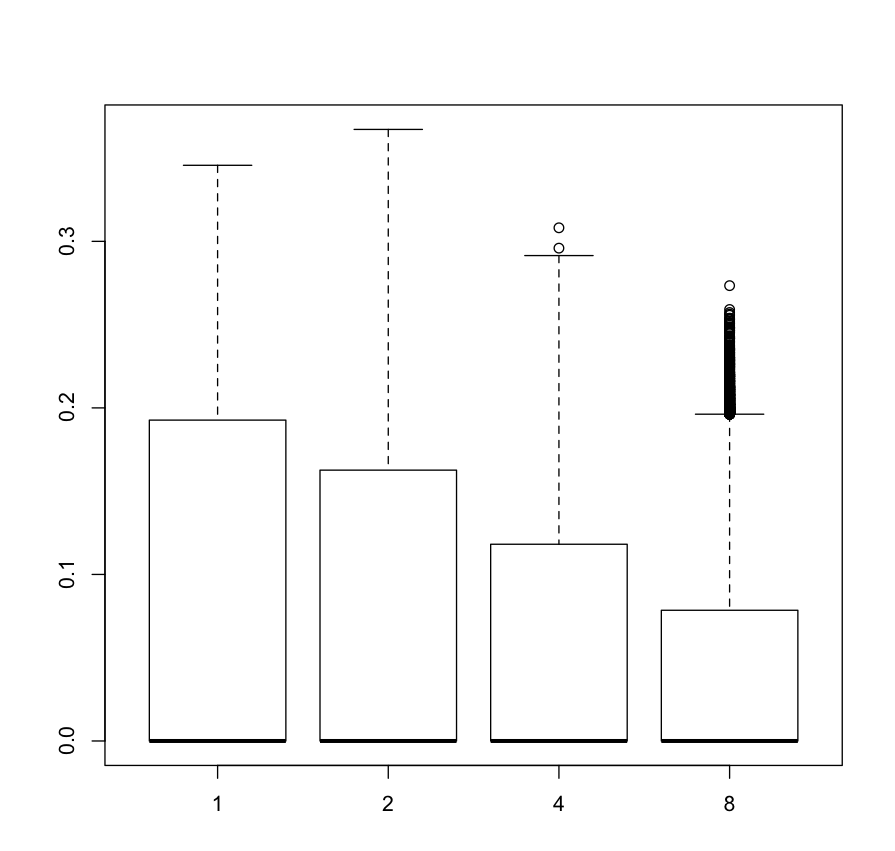
\includegraphics[width=3.5cm]{imags/e1_p.png}
                \label{fig:e1_p}
        }
        \subfigure[Days]{
                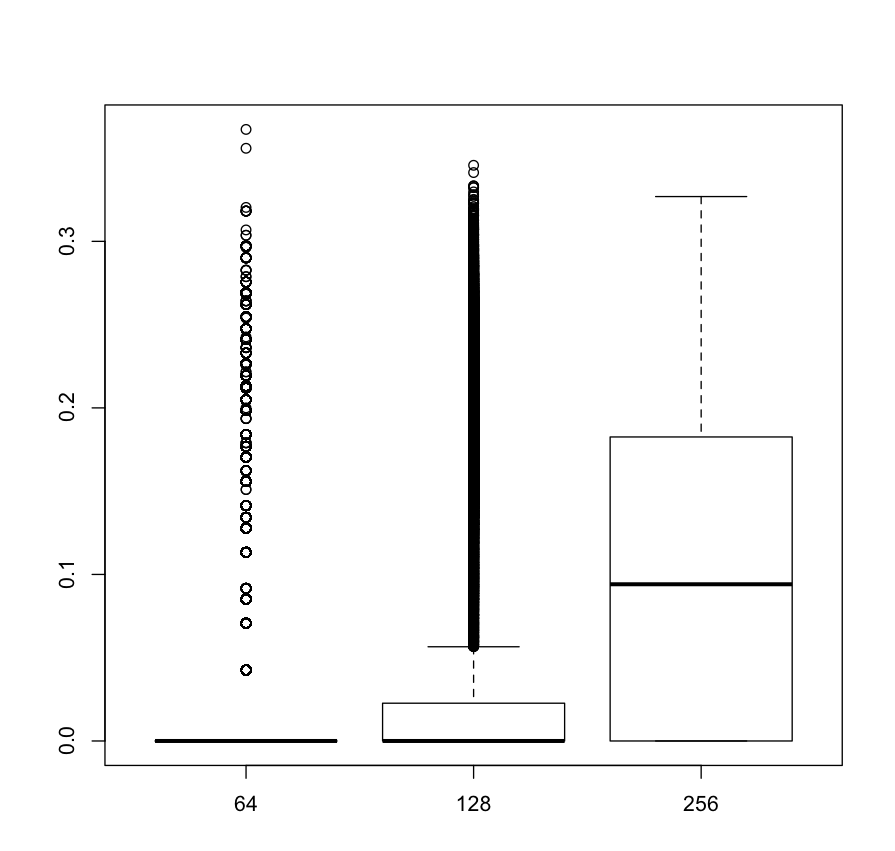
\includegraphics[width=3.5cm]{imags/e1_d.png}
                \label{fig:e1_d}
        }
        \subfigure[World Size]{
                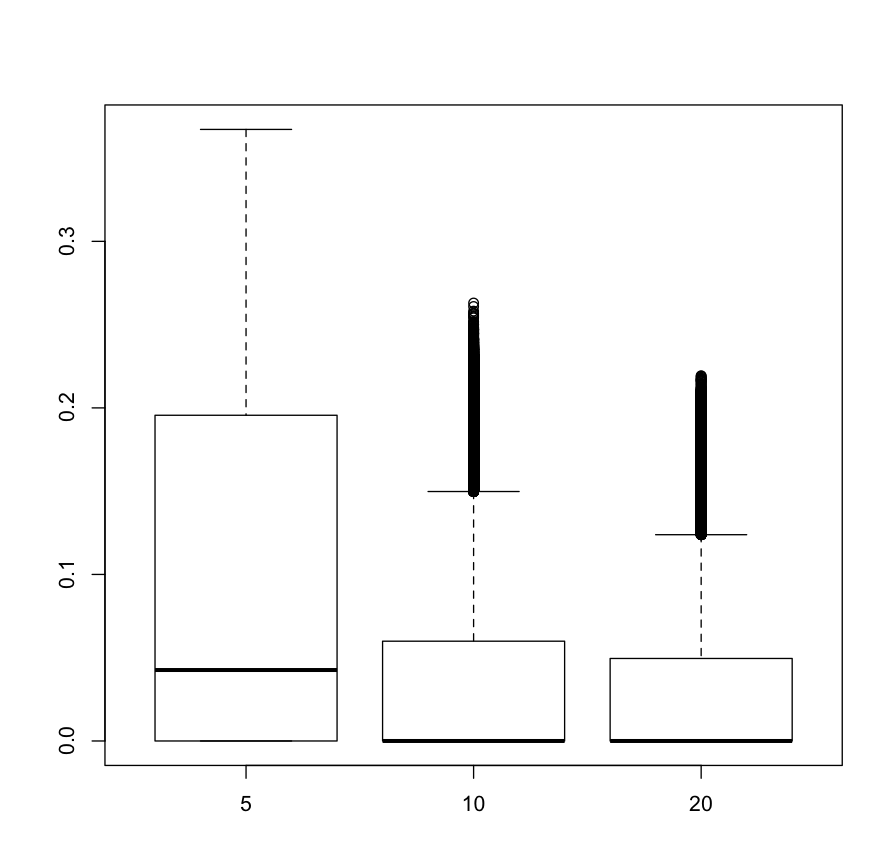
\includegraphics[width=3.5cm]{imags/e1_w.png}
                \label{fig:e1_w}
        }  
        \subfigure[Food]{
                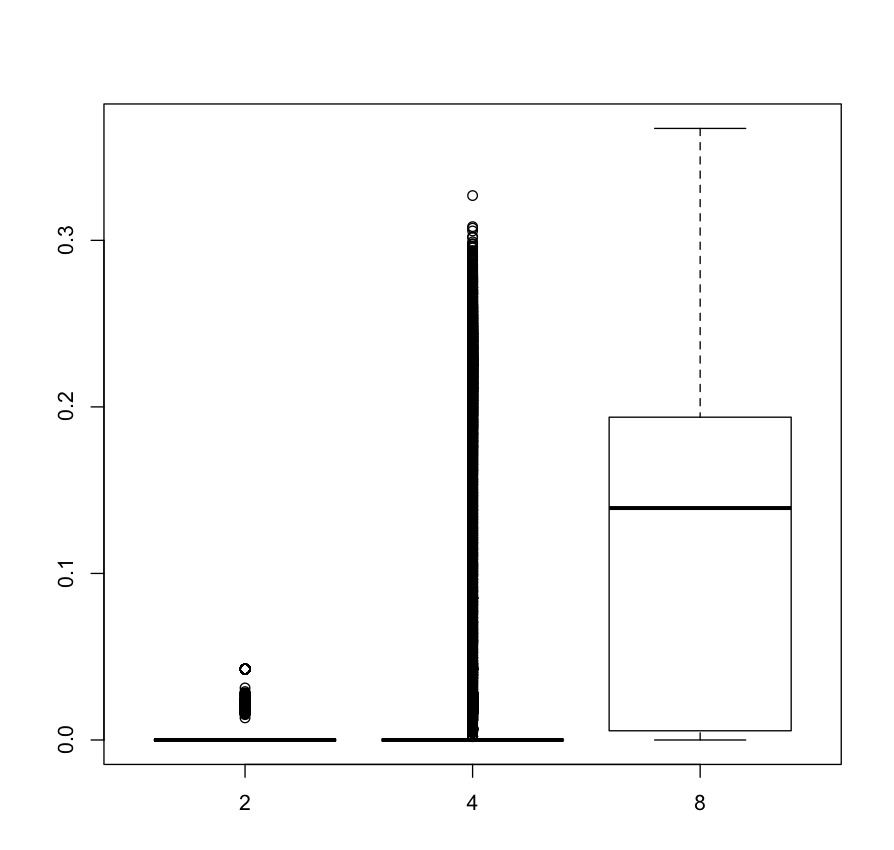
\includegraphics[width=3.5cm]{imags/e1_f.png}
                \label{fig:e1_f}
        }
        \subfigure[Population Size]{
                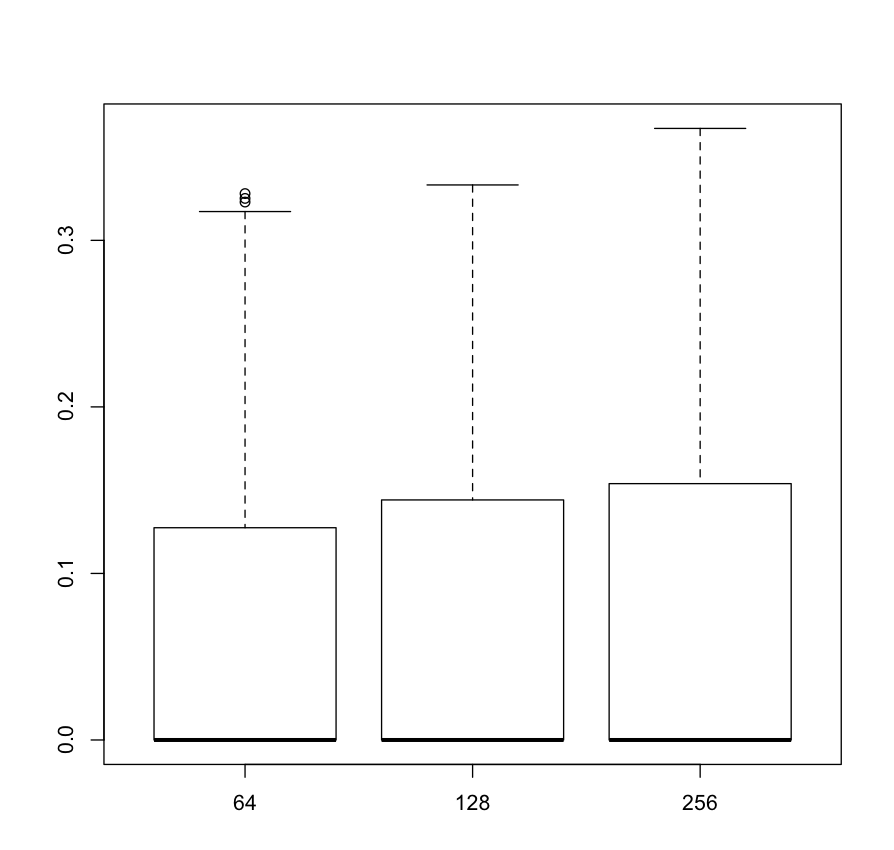
\includegraphics[width=3.5cm]{imags/e1_s.png}
                \label{fig:e1_s}
        }

        \caption{Boxplots for scenario E1}\label{fig:boxplotsE1}
\end{figure}

\begin{figure}
        \centering
        \subfigure[Profiles]{
                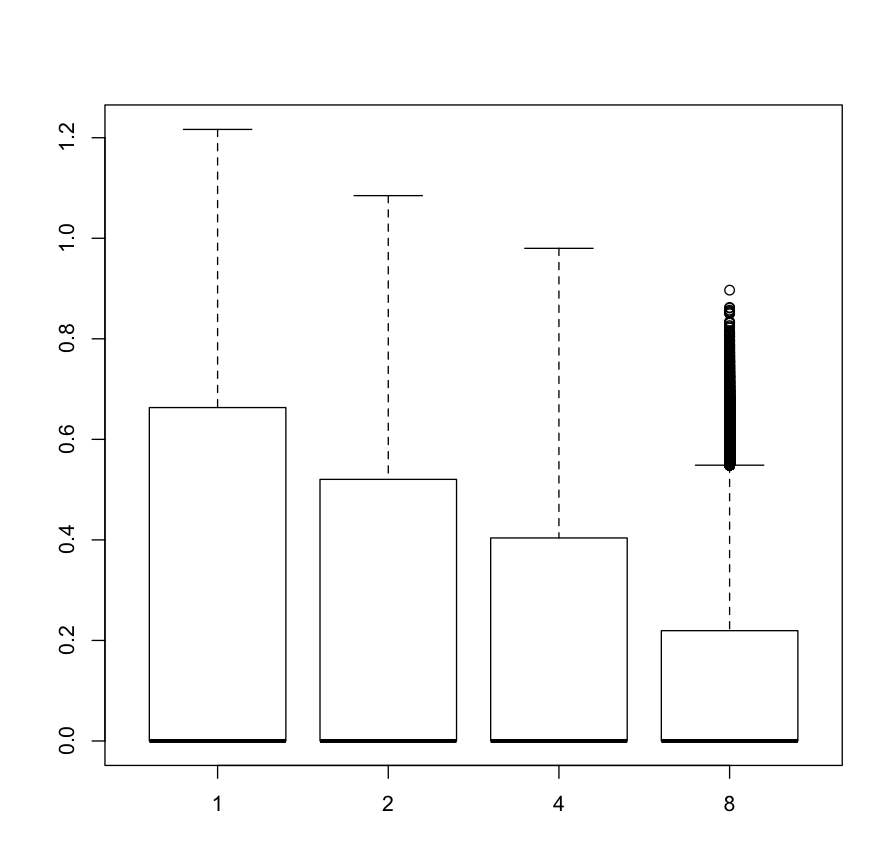
\includegraphics[width=3.5cm]{imags/e2_p.png}
                \label{fig:e2_p}
        }
        \subfigure[Days]{
                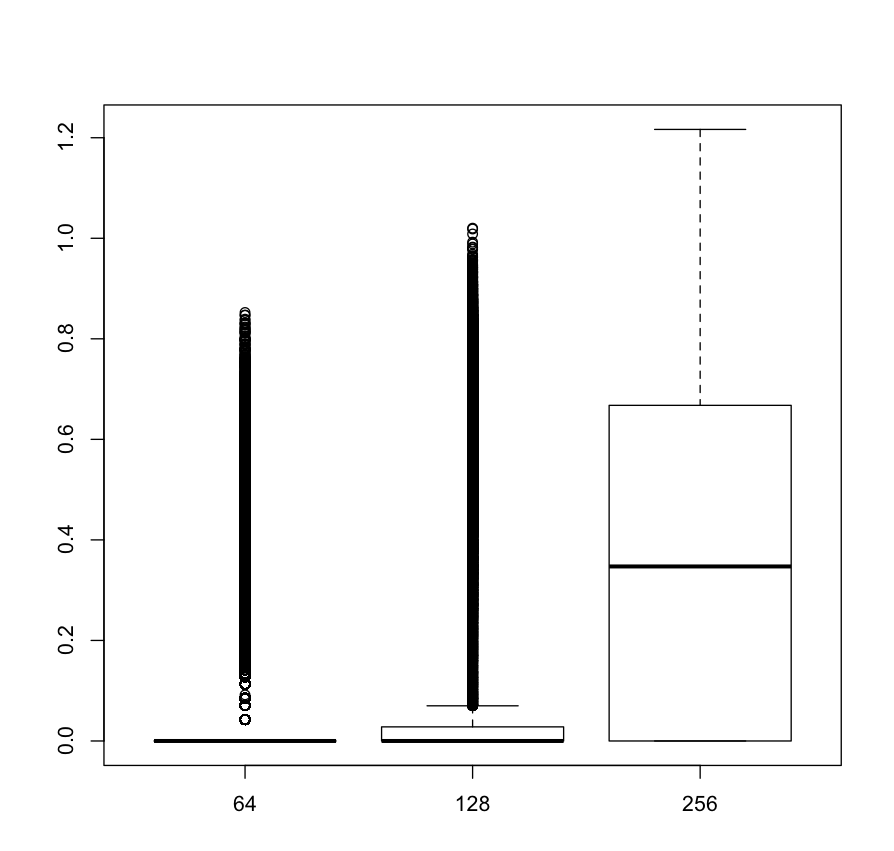
\includegraphics[width=3.5cm]{imags/e2_d.png}
                \label{fig:e2_d}
        }
        \subfigure[World Size]{
                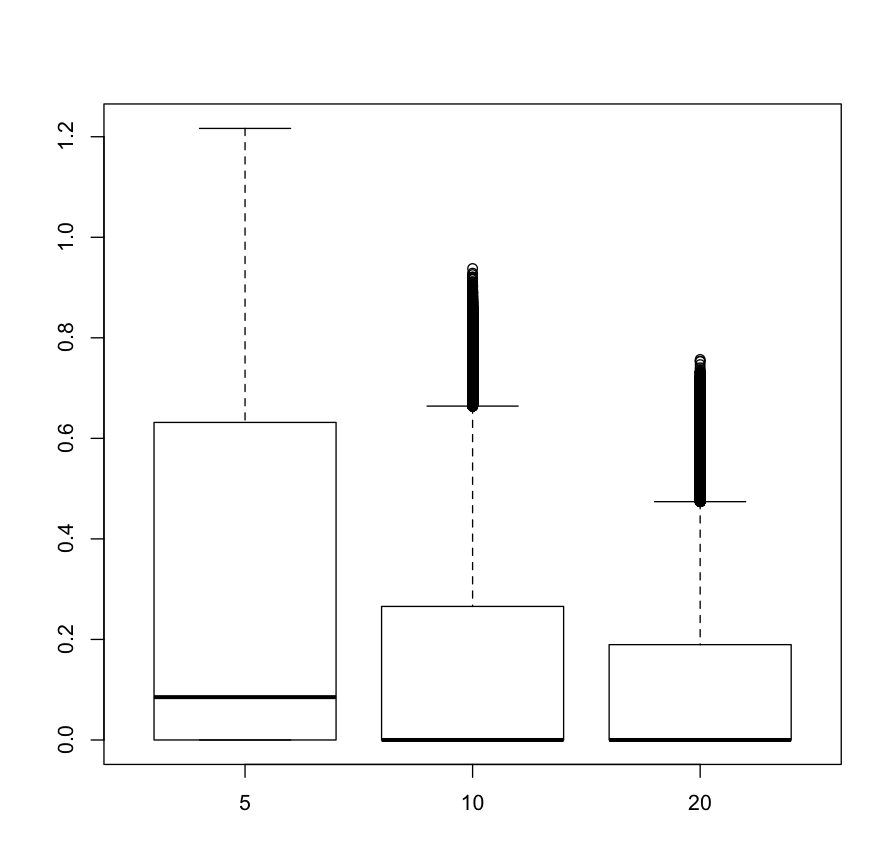
\includegraphics[width=3.5cm]{imags/e2_w.png}
                \label{fig:e2_w}
        }  
        \subfigure[Food]{
                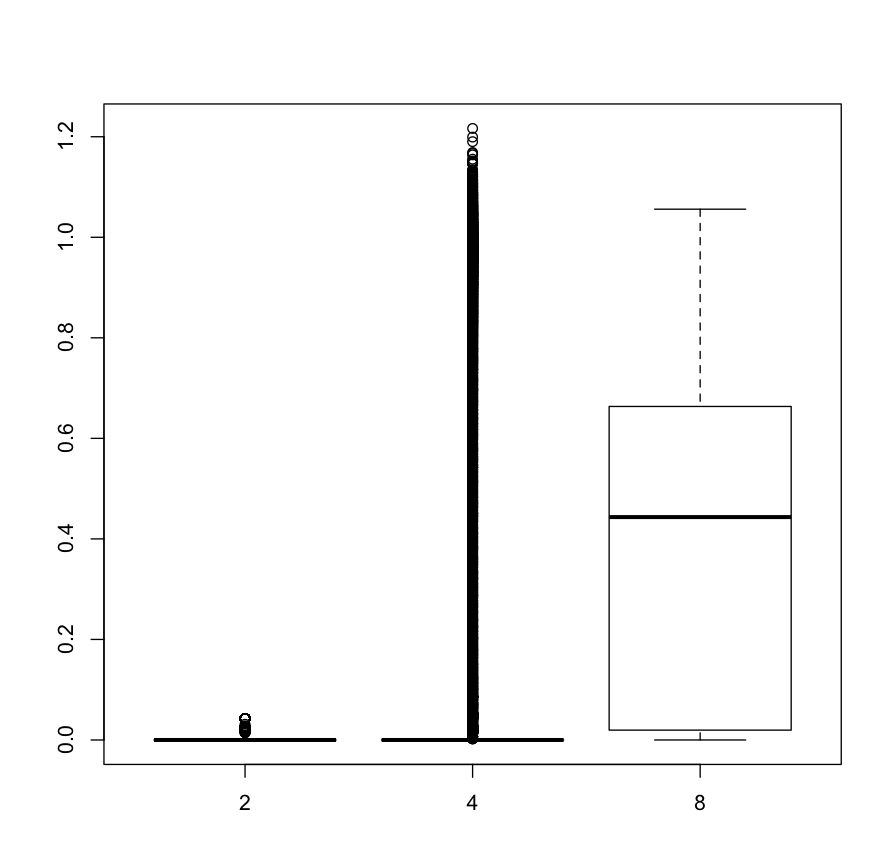
\includegraphics[width=3.5cm]{imags/e2_f.png}
                \label{fig:e2_f}
        }
        \subfigure[Population Size]{
                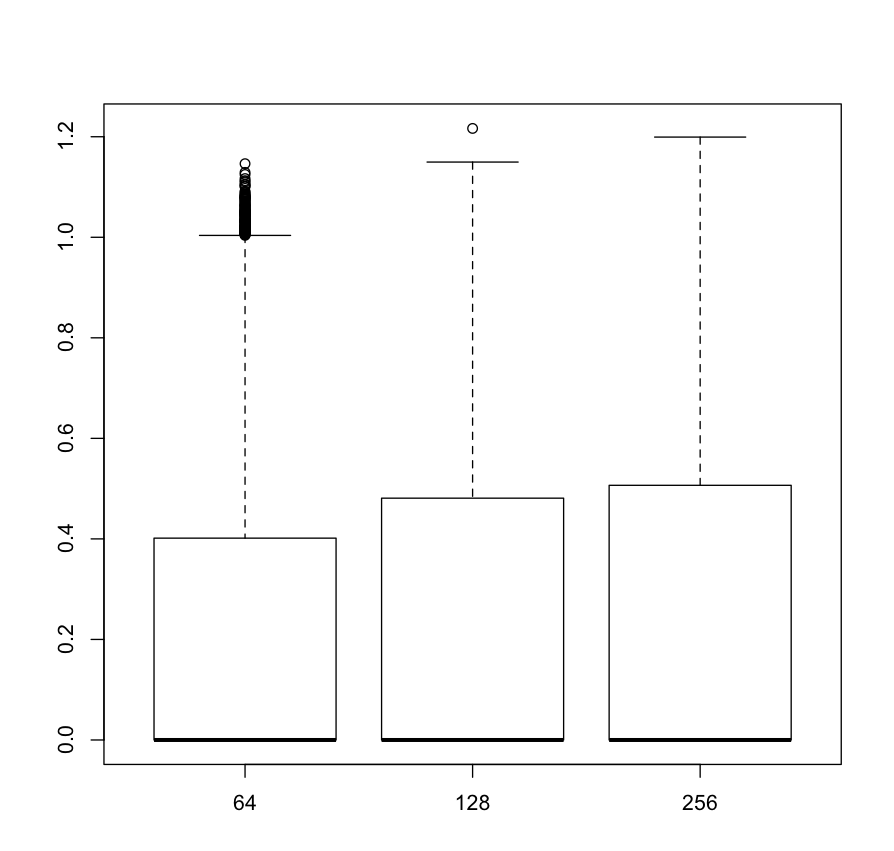
\includegraphics[width=3.5cm]{imags/e2_s.png}
                \label{fig:e2_s}
        }

        \caption{Boxplots for scenario E2}\label{fig:boxplotsE2}
\end{figure}

\begin{figure}
        \centering
        \subfigure[Profiles]{
                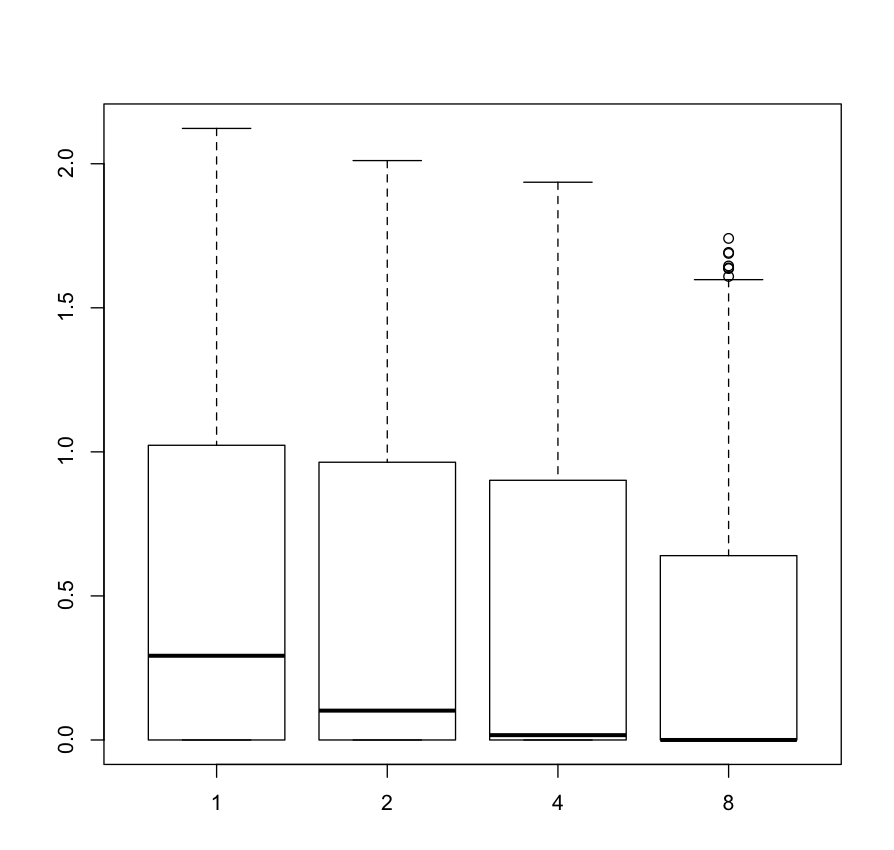
\includegraphics[width=3.5cm]{imags/e5_p.png}
                \label{fig:e5_p}
        }
        \subfigure[Days]{
                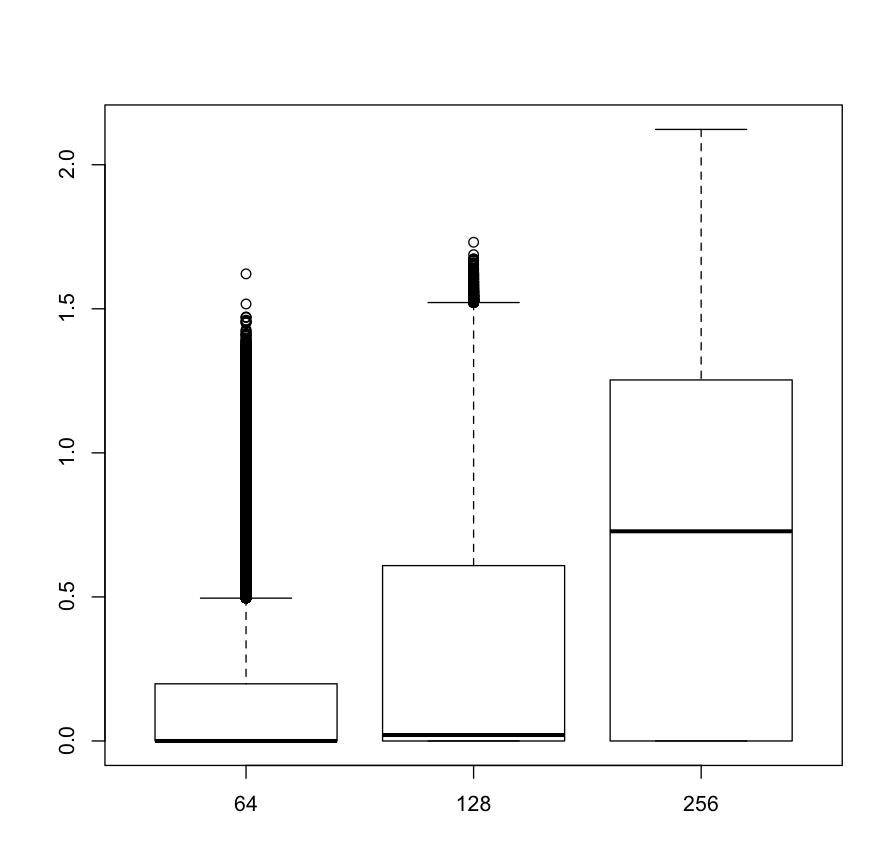
\includegraphics[width=3.5cm]{imags/e5_d.png}
                \label{fig:e5_d}
        }
        \subfigure[World Size]{
                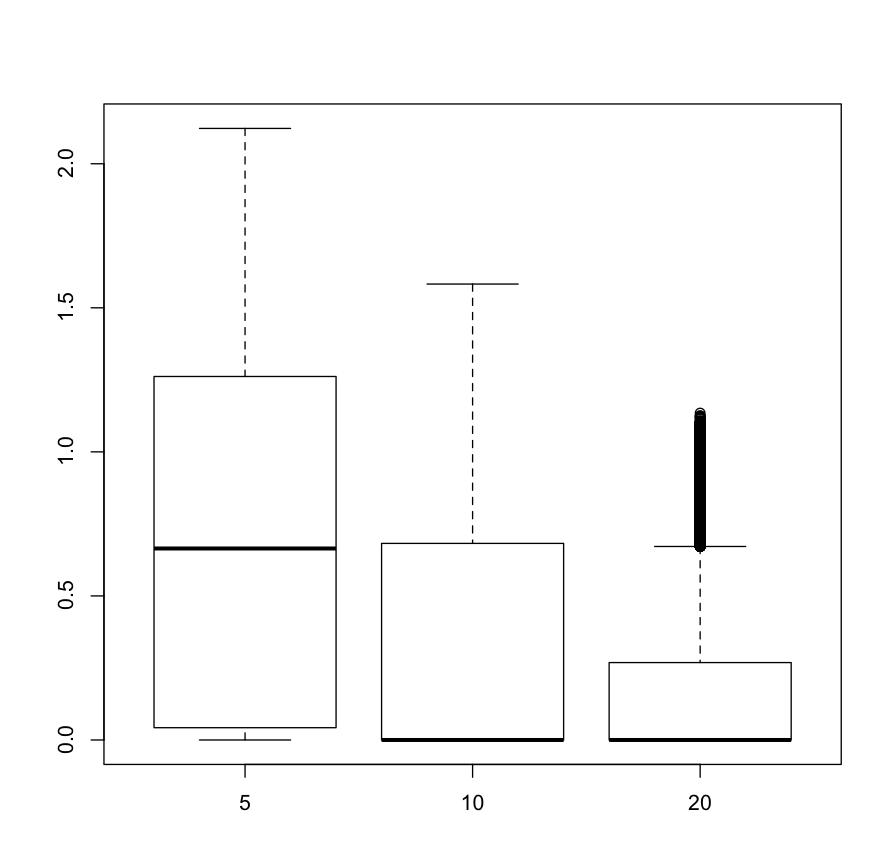
\includegraphics[width=3.5cm]{imags/e5_w.png}
                \label{fig:e5_w}
        }  
        \subfigure[Food]{
                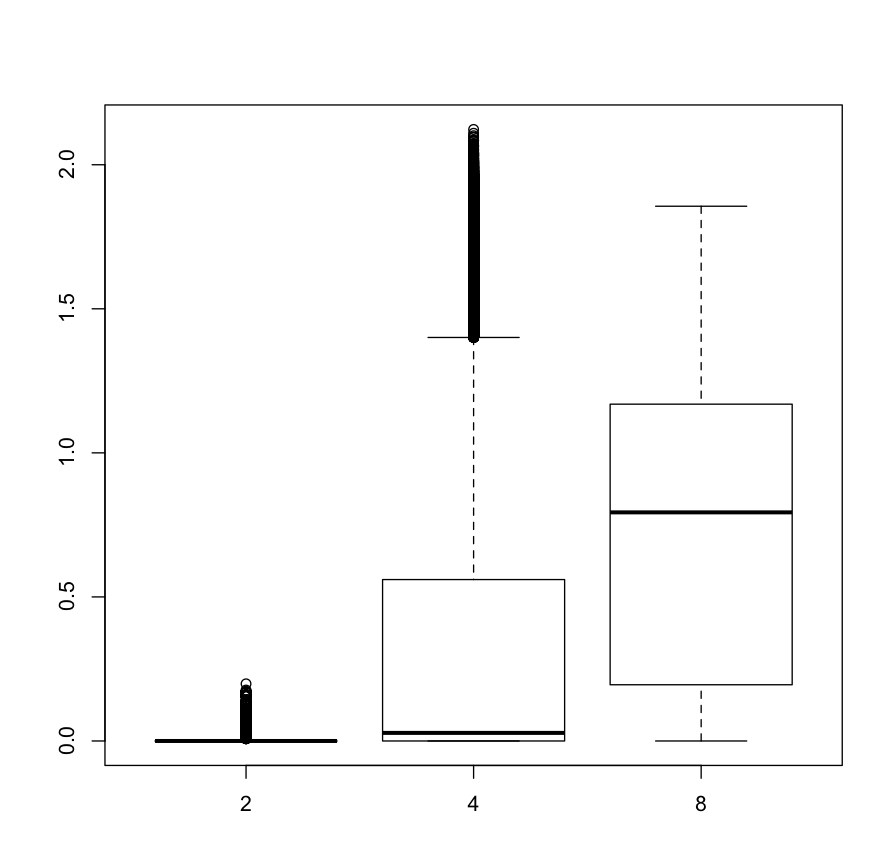
\includegraphics[width=3.5cm]{imags/e5_f.png}
                \label{fig:e5_f}
        }
        \subfigure[Population Size]{
                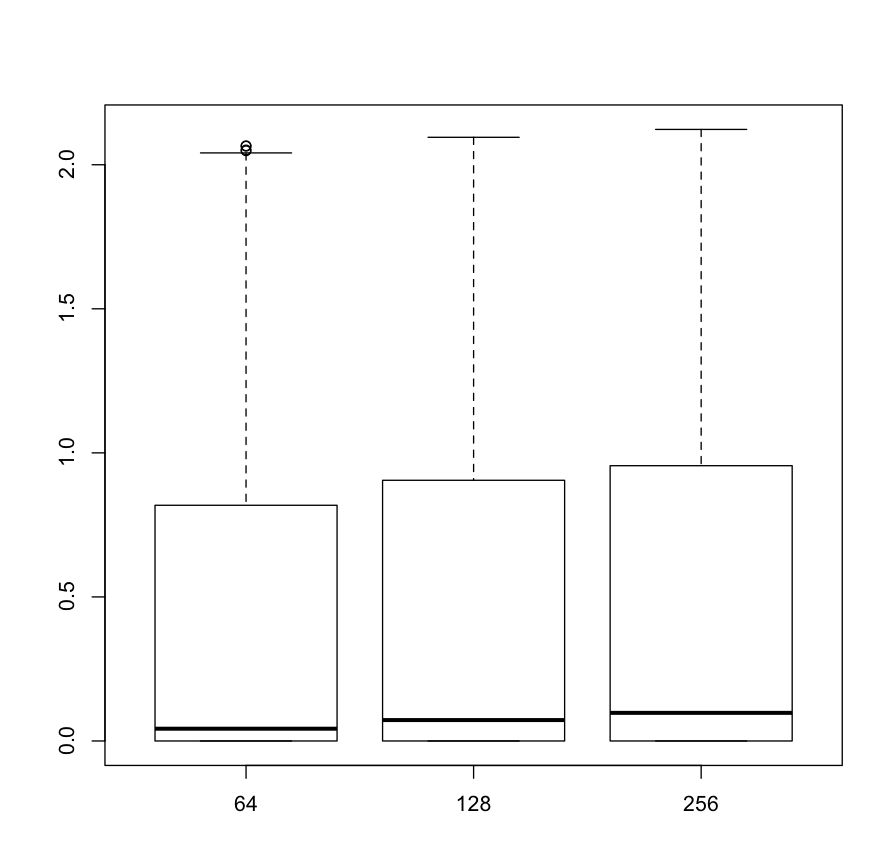
\includegraphics[width=3.5cm]{imags/e5_s.png}
                \label{fig:e5_s}
        }

        \caption{Boxplots for scenario E5}\label{fig:boxplotsE5}
\end{figure}


\section{Conclusions}

\section*{Acknowledgements}

Hidden for double-blind review

\bibliographystyle{unsrt}
\bibliography{geneura,references}

\end{document}
